\section{Computational complexity}
Let us define some notation:
\begin{defn}[Big $\mathbb{O}$ notation]
   Let $f$ be a real or complex valued function and $g$ a real valued function. Let both functions be defined on some unbounded subset of positive real numbers. One writes
   \begin{equation*}
       f(x) = \mathbb{O}(g(x)) \quad \text{as} \quad x \rightarrow a
   \end{equation*}
   if 
   \begin{equation*}
      \lim_{x \to a} \sup{\frac{\abs{f(x)}}{g(x)}} < \infty
   \end{equation*}
   \end{defn}
   \begin{defn}[Big $\Omega$ Knuth notation]
      Let $f$ be a real or complex valued function and $g$ a real valued function. Let both functions be defined on some unbounded subset of positive real numbers. One writes
   \begin{equation*}
       f(x) = \Omega(g(x))
    \Longleftrightarrow
      g(x) = \mathbb{O}(f(x)).
   \end{equation*}
   \end{defn}
   

\subsection{Performance}\label{sec:performance}
Following the geometric interpretation of section~\ref{sec:geometric-interpretation} we are going to calculate the number of iterations $R$ necessary for the algorithm to find the solution. The initial state of the system is~\ref{eq:initial-state} so rotating through $\arccos{\sqrt{M/N}}$ radians to take the system to $\ket{\beta}$.
\begin{defn}
$\text{CI}(x)$ denote the integer closest to the real number $x$, rounded halves down.
\end{defn}
Then repeating the Grover iteration:
\begin{equation}\label{eq:R}
    R = \text{CI}\biggl(\frac{\arccos{M/N}}{\theta}\biggr)
\end{equation}
times rotates $\ket{\psi}$ to within an angle $\theta/2 \leq \pi/4$ of $\ket{\beta}$. Recalling the state~\ref{eq:initial-state} we can see that observation of the state in the computational basis yields a solution with a probability at least $1/2$. 

When $M<<N$ we have\footnote{\label{foot:sin}We can demonstrate that $\sin\theta = 2\sqrt{M(N-M)}/N$.} $\theta \approx \sin\theta \approx 2\sqrt{M/N}$ an thus the angular error in the final state,, recalling again the state~\ref{eq:initial-state}, is at most $\theta/2 \approx \sqrt{M/N}$; giving a probability of error of at most $M/N$.

We can find an upper bond for R. Note from \ref{eq:R}  that R has an upper bound $R \leq \pi/2\theta$, let us find now a lower bound on $\theta$, assuming that\footnote{We are going to discuss this limit in section~\ref{sec:M}.} $M \leq N/2$ we have:
\begin{equation*}
    \frac{\theta}{2} \geq \sin\frac{\theta}{2} = \sqrt{\frac{M}{N}}
\end{equation*}
from which we can obtain an upper bound on the number of iterations required,
\begin{equation}\label{eq:upper-bound}
    R \leq \frac{\pi}{4} \sqrt{\frac{N}{M}}.
\end{equation}
That is, $R = \mathbb{O}(\sqrt{N/M})$ $G$ iterations (and thus oracle calls) must be performed in order to obtain a solution with high probability, a quadratic improvement over the $\mathbb{O}(N/M)$ oracle calls required classically.

\subsection{Number of solutions}\label{sec:M}
Until now we assumed that $M\leq N/2$; if $M \geq N/2$ from the expression\footnote{See footnote~\ref{foot:sin}.} $\theta=\arcsin(2\sqrt{M(N-M)}/M)$ we can see that $\theta$ get smaller as $M$ increase from $N/2$ to $N$. And then we see from~\ref{eq:R} the number of iterations needed by the search algorithm increases with $M$, for $M\geq N/2$.

We can distinguish two scenarios:
\begin{description}
   \item[$M$ is known] If $M$ is known in advance to be larger than $N/2$ then we can just randomly pick an item from the search space, and then check that it is a solution using the subroutine. This approach has a success probability at least one-half, and only requires one consultation with the oracle.
   \item[$M$ is not known] In the case where it isn't known whether $M\geq N/2$ we double the number of elements in the search space by adding $N$ extra items to the search space, none of which are solutions. We can do that adding a single qubit $\ket{x'}$ to the search index, doubling the number of items to be searched to $2N$. A new augmented subroutine $\hat{U'}_\beta$ which marks an item only if it is a solution to the search problem and the extra bit is set to zero. The new search problem has then $M \leq 2N$ solutions and therefore running the algorithm with the subroutine $\hat{U'}_\beta$ at most $R$, as defined in~\ref{eq:upper-bound}, calls to the subroutine are required, and it follows that $\mathbb{O}(N/M)$ calls to $\hat{U}_\beta$ are required to perform the search.
\end{description}
\subsection{Optimality of the search algorithm}
We shall show that no quantum algorithm can perform the task of searching through $N$ unsorted items using fewer than $\Omega(\sqrt{n})$ access to the subroutine\footnote{Again we restrict ourself in the case $M=1$.}:
\begin{theorem}
The quantum search algorithm is optimal. 
\end{theorem}
\begin{proof}
TODO [...]

To achieve a probability of success at least $1/2$ for finding a solution to the search problem we must call the oracle $\Omega(\sqrt{N})$ times.
\end{proof}

\subsection{Quantum computational complexity}
We take for granted some basic definitions of classical computational complexity theory and we proceed defying
\begin{defn}
\textbf{BPP} is the class of languages that can be solved in polynomial time by probabilistic Turing machines with error probability bounded by $1/3$. Using standard boosting techniques the error probability can then be made exponentially small in $k$ by iterating the algorithm $k$ times.
\end{defn}
\begin{defn}
\textbf{PSPACE} is the class of languages that may be solved on a Turing machine using a polynomial number of working bits, with no limitations on the amount of time that may be used by the machine.
\end{defn}
\begin{defn}
\textbf{BPQ} is the class of languages that can be solved in polynomial time by quantum Turing machines with error probability bounded by $1/3$. The error probability can be made exponentially small as in \textbf{BPP}.
\end{defn}
There are some evidence~\cite{Bennett_1997} that $\textbf{BQP} \neq \textbf{BPP}$ (i.e. polynomial-time quantum Turing machines are more powerful than polynomial-time probabilistic Turing machines). Since \textbf{BPP} is regarded as the class of all efficiently computable languages, this provides evidence that quantum computers could be inherently more powerful than classical computers in a model-independent way.

However exactly where \textbf{BQP} fits with respect to \textbf{P}, \textbf{NP} and \textbf{PSPACE} is as yet unknown. What is known is that quantum computers can solve all the problems in \textbf{P} efficiently and that there are no problems outside of \textbf{PSPACE} which they can solve efficiently. Therefore, \textbf{BQP} lies somewhere between \textbf{P} and \textbf{PSPACE}.
Proving that $\textbf{BQP} \neq \textbf{BPP}$ would definitively establish that $\textbf{P} \neq \textbf{PSPACE}$ solving a major problem in computer science.


\begin{figure}
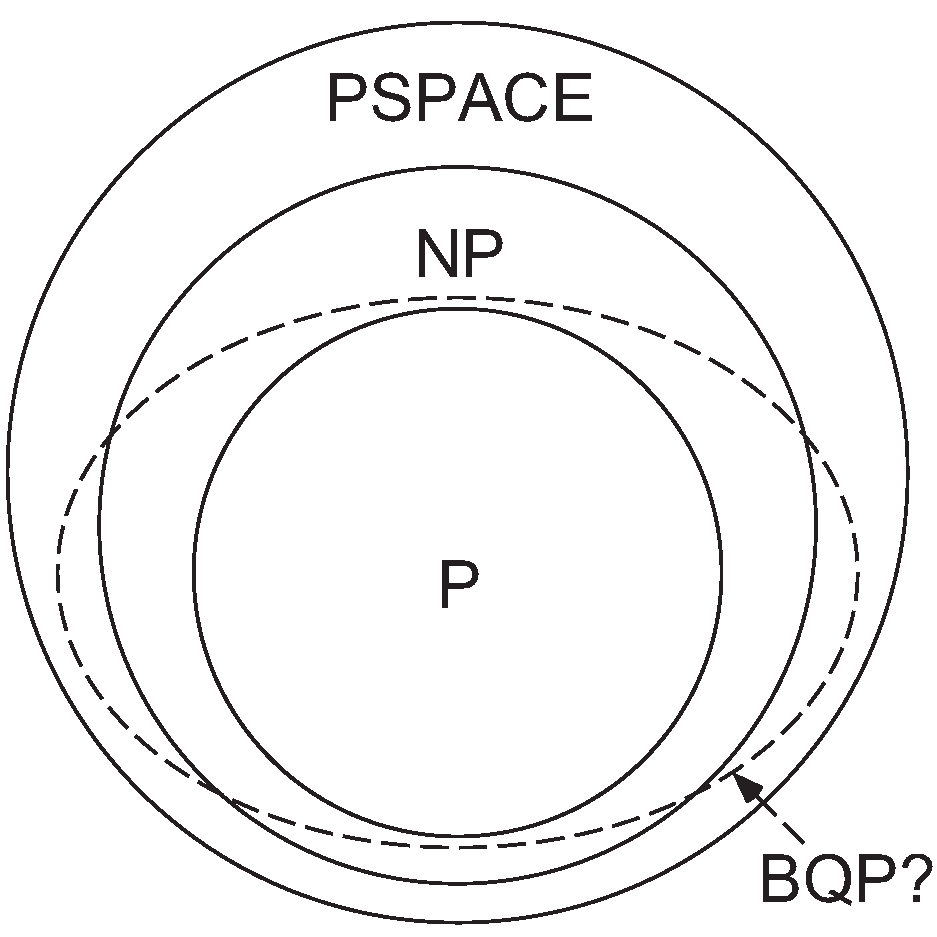
\includegraphics{computational-complexity.png}
\centering
\caption{The relationship between classical and quantum complexity classes.}
\end{figure}
We know that we can transform \textbf{NP}-complete problems into Grover-type search problems.
The fact that the quantum search algorithm is optimal means that it is not possible to search an $N$ item search space using $\mathbb{O}(\log_2{N})$ calls of $\hat{U}_\beta$. If such an algorithm existed, it would allow us to solve \textbf{NP}-complete problems efficiently on a quantum computer.

This does not rule out the possibility that \textbf{NP} $\subseteq$ \textbf{BQP}. What this result do establish is that there is no a search-based method for attacking \textbf{NP}-complete problems.
However we note that many researchers believe that the search space of \textbf{NP}-complete problems has no structure and that the best possible method for solving such problems is to adopt a search method. If one takes this point of view this indicates that \textbf{BQP} does not contain the \textbf{NP}-complete problems.